\documentclass[draft]{report}

\usepackage{graphicx}
\usepackage{siunitx}
\sisetup{
  round-mode = places,
  round-precision = 3
}

% Insert a results file
\newcommand{\results}[1]{\begin{tabular}{lll}
                           \beginrule
                           \midrule
                           \input{#1}
                           \endrule
                         \end{tabular}}
% format a result
\newcommand{\runsummary}[3]{}
\newcommand{\result}[3]{#1 & #2 & #3\\}
% Format each result record
\newenvironment{resultashdfksj}[2]{\item #2 \hfill{\small (\num{#1})}\begin{quote}}{\end{quote}}

% name
\newcommand{\pagerank}{PageRank }
\newcommand{\pageranks}{PageRanks }

\title{CPE466\\Lab3}
\author{
  Gilbert, Andrew\\
  \texttt{apgilber@calpoly.edu}
  \and
  Terrell, Josh\\
  \texttt{jmterrel@calpoly.edu}
}
\date{}

\begin{document}

\maketitle

\begin{abstract}
When working with a graph of social data, where nodes represent actors and edges
represent relationships, it can be useful to determine the most influential
nodes. The \pagerank algorithm provides a straightforward way to rank nodes based
on their influence. We implemented the \pagerank algorithm and observed its
results on various datasets.
\end{abstract}

\section{Introduction}
The \pagerank algorithm, developed by Larry Page and Sergey Brin, and initially
used in what became the Google search engine, is a technique for calculating the
importance of nodes in a graph. We wrote and tested an implementation of this
algorithm to better understand how it works as well as observe its behavior on
various datasets.

\section{Implementation Overview}
We implemented our reading and writing system in Python. We wrote the
\pagerank algorithm in c, and used Python's cffi library to interface between
the two languages.

The ranking process starts by loading a given file into memory by parsing each
line as an edge between two nodes. Each edge can have an optional weight. If the
\texttt{--weighted} flag is specified, the weight is read from file. Otherwise
each line is expected to be an edge between the left node pointing to the right
node.

Our implementation computes the standard \pagerank with options to customize its
behavior: 

\begin{list}{}{}
  \item \texttt{--help} --- display all the below options and descriptions
  \item \texttt{--dval <int>} --- the \texttt{d} parameter of the \pagerank
  algorithm; probability of following a link
  \item \texttt{--epsilon <float>} --- (per iteration) consider the algorithm to
  have converged if the maximum change in \pagerank of each node in the graph is
  less than epsilon
  \item \texttt{--maxiterations <int>} --- the number of iterations the algorithm
  will run before before giving up and considering the graph converged
  \item \texttt{--threads <int>} --- the number of computation threads to use
  \item \texttt{--batchsize <int>} --- per iteration, each thread claims
  \texttt{batchsize} nodes at a time to compute \pagerank for. Too small and the
  threads will spend all their time synchronizing around a mutex. Too large and
  all the threads may wait on one thread to finish so the algorithm can continue
  to the next iteration.
  \item \texttt{--fmt string} --- the data format; either csv (default) or snap
  \item \texttt{--scale} --- scale epsilon and the printed results by the size of
  the graph.
  \item \textbf{\texttt{--weighted}} --- specify if the graph includes weights per
  edge.
\end{list}

When the \texttt{--weighted} flag is enabled, our algorithm runs a modified
version of \pagerank which takes into account the weights of edges. The modified
version computes \pagerank such that the weight is the number of edges between
the nodes. The result is that edges with higher weight indicate stronger
relationships than edges with lower weights.

The in-memory representation of the graph, \pagerank computation, and parallel
execution all happen in c. In the parallelized \pagerank computation, each thread
asks the master thread for a block of nodes to work on. Each node has two page
ranks---the page rank of the previous iteration and the page rank of this
iteration.  By having both page ranks, we were able to parallelize computation
without forcing Nodes to be computed in a specific order.

The graph is composed of an array of Nodes, a c structure with six fields:
\begin{lstlisting}[language=C]
{
  unsigned int id;
  char active;
  double pageRank_a;
  double pageRank_b;
  int outDegree;
  struct LLNode *inNodes;
}
\end{lstlisting}

The \pagerank fields allow us to switch between the page rank of the last
iteration and this iteration. inNodes is a linked list of incomming edges. Each
edge has a source node and weight.

Once the graph is built, many iterations of the \pagerank are computed until the
algorithm converges. On every iteration, worker threads calculate \pagerank
on blocks of nodes from the list of nodes that haven't been processed yet until
there are no nodes left to process in the iteration.

For each node in the block, the current \pagerank is read from either the
\texttt{pageRank\_a} or \texttt{pageRank\_b} field and the new rank is written
to the other. If the rank has changed more than the (configurable) epsilon, a
flag is updated to inform the system that the algorithm has not converged. Once
all the worker threads have completed their work, if the ``unconverged'' flag is
set, the master thread starts the workers again, this time telling them to read
from the field they were just writing to and to write to the field they were
reading from.

\section{Results}
\subsection{STATES}
\results{stateborders-results.tex}
\subsection{NCAA-FOOTBALL}
We observered that the NCAA data set is troublesome to run as unweighted because
the nodes are in the opposite order from the other datasets. Typically edges in
the dataset run from left (source) to right (destination), but for \pagerank to
do anything meaningful with this dataset, the edges must run from right to left.
This is because the left team is always the winning team, and thus there should
be an edge connecting from losing team (right) to winning team (left) to
represent the winning team gaining prestige from the losing team. Our program
only provides meaningful results for this dataset if the \texttt{--weighted}
flag is provided, in which case the edges are flipped to go from right to left
due to the weighting of edges.

\results{NCAA_football-results.tex}
\subsection{KARATE}
\results{karate-results.tex}
\subsection{DOLPHINS}
\results{dolphins-results.tex}
\subsection{LES-MISERABLES}
\results{lesmis-results.tex}
%\input{lesmistimes.tex}
\subsection{POLITICAL-BLOGS}
\results{polblogs-results.tex}
\subsection{WIKI-VOTE}
\results{wiki-Vote-results.tex}
\subsection{P2P-GNUTELLA05}
\results{p2p-Gnutella05-results.tex}
\subsection{SLASHDOT-ZOO-NOV6-2008}
\results{soc-sign-Slashdot081106-results.tex}
\subsection{AMAZON-MAY03}
\results{amazon0505-results.tex}
\subsection{LIVEJOURNAL1}
\results{soc-LiveJournal1-results.tex}

\section{Overall Summary}
Before implementing edge weights, page rank appeared to do decently on the
graphs we manually tested. We created our own fakeball dataset, and analyzed
carefully the results of the NCAA football dataset before and after weighting.
As noted in the NCAA football section of Results, NCAA football was a bit
troublesome to run unweighted.

Once we implemented edge weights, we noticed different rankings of the football
teams, and the change in rankings seemed a bit more inline with the rankings
from ESPN's 2008 data, though the rankings were far from perfect. We also
compared the \pagerank results with a ranking the teams by total score. Weighted
\pagerank matched much more closely to the teams sorted by total season score.

\section{Performance Evaluation}
All datasets were successfully executed in under 30 minutes (combined) on a 4-core hyperthreaded processor using 8 threads. The execution time for each dataset is provided in \cref{execution-times-table}. A visual representation is also included in \cref{execution-times-graph}. Note that that on the graph, both the x and y axis are drawn in log10 so the outliers do not croud out the trends. The visible trend on the graph suggests that the execution times increase roughly linearly as edge count increases to the max of our dataset.  

\begin{table}
  \centering
  \begin{tabular}{ll}
    \toprule
    Dataset & Execution Time (seconds)\\
    \midrule
    amazon0505 & 38.734575 \\
    dolphins & 0.005477999999999997 \\
    karate & 0.004890999999999993 \\
    lesmis & 0.005057000000000006 \\
    NCAA\_football & 0.006725000000000009 \\
    p2p-Gnutella05 & 0.025919000000000025 \\
    polblogs & 0.06062600000000001 \\
    soc-LiveJournal1 & 1121.060663 \\
    soc-sign-Slashdot081106 & 2.5643610000000003 \\
    stateborders & 0.006414000000000003 \\
    wiki-Vote & 0.0008580000000000254 \\
    \bottomrule
  \end{tabular}
  \caption{Execution Times on Datasets}
  \label{execution-times-table}
\end{table}
\begin{figure}
  \centering
  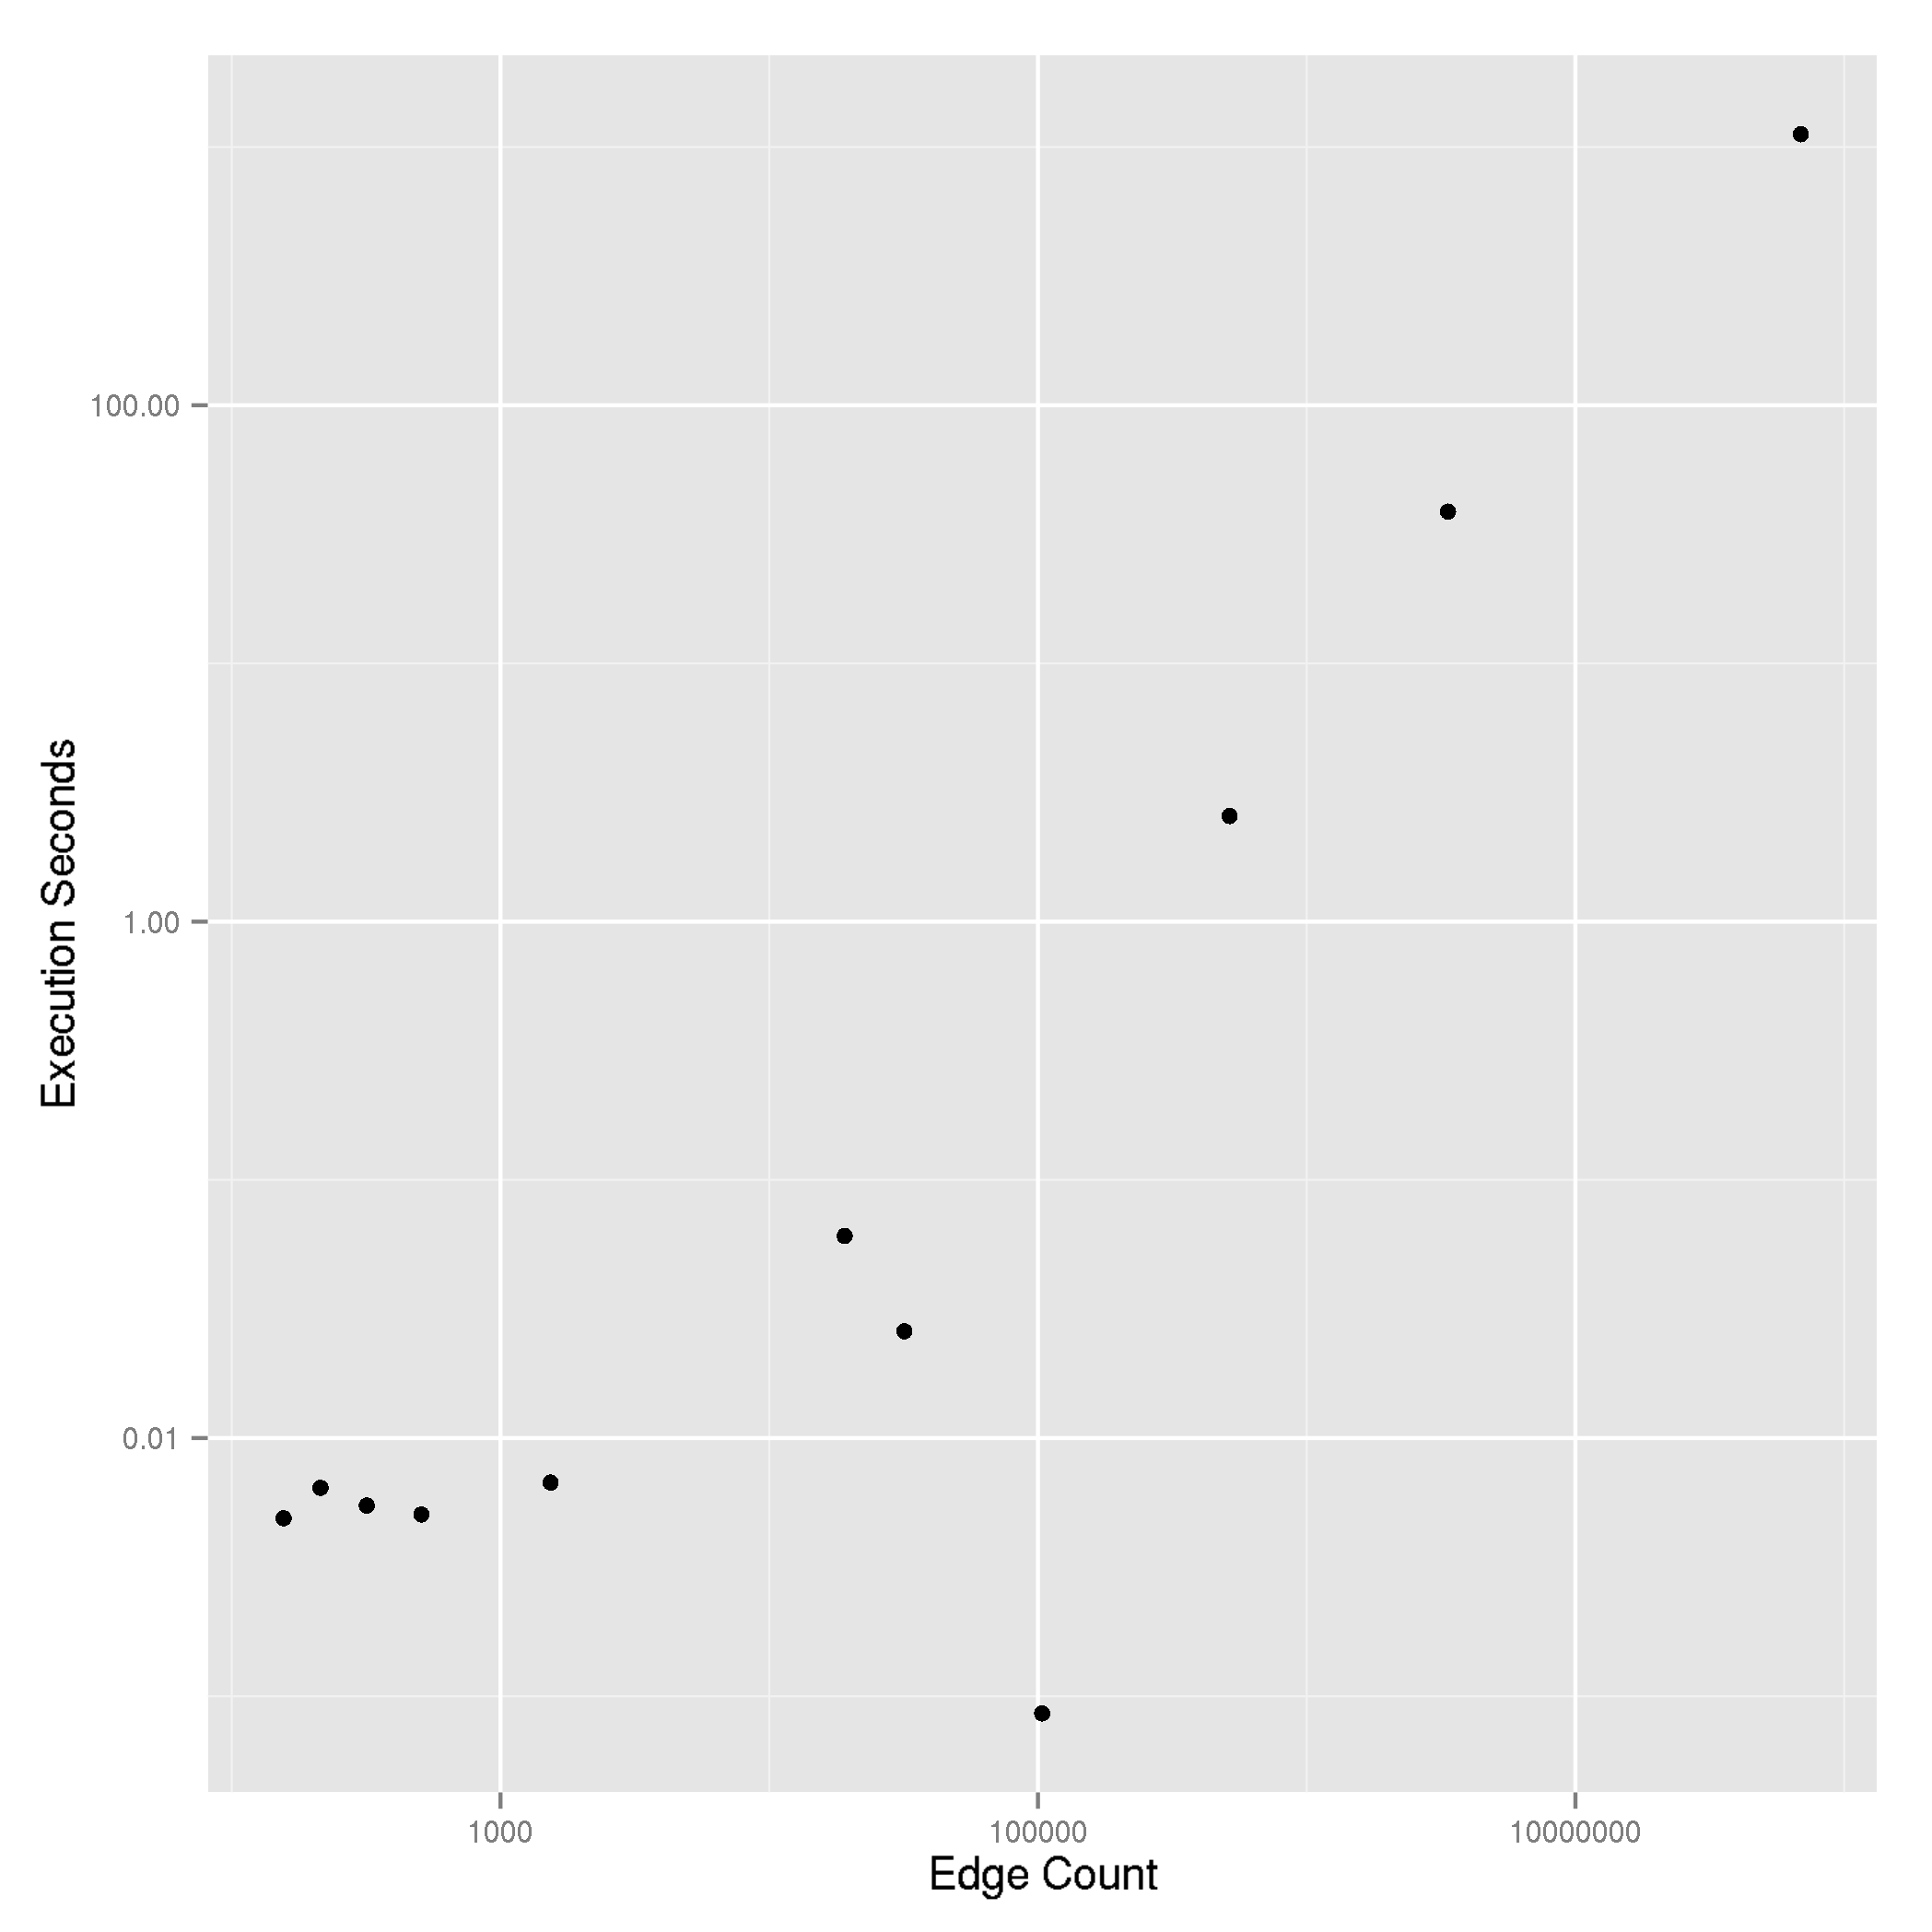
\includegraphics[scale=0.5]{performance.png}
  \caption{Graph of Execution Times on Datasets}
  \label{execution-times-graph}
\end{figure}

\section{Extra Credit}
We added a weighted flag to our algorithm which takes into account a weight per
edge when computing \pagerank. We experimented with different ideas, but decided
that simply using the weight as a multiplication factor for the importance of
the edge would have the desired effect. We treated weights as edge counts.  For
instance, if the edge a->b had a weight of 7, we would compute page rank as if
there were 7 edges from a to b. A weight of -7 would mean there were 7 edges in
the opposite direction.

Increasing the edges also involved increasing the node count. We discovered that
\pagerank would not converge unless we added an appropriate amount of fake nodes
to the graph so that outdegree and other variables of the \pagerank computation
were accurate.

We used our weighted modification to the \pagerank algorithm to compute \pageranks
for the NCAA\_football, lesmis, and SlashDot datasets.


\appendix

\section{README}
\lstset{language=bash}
Team: Andrew Gilbert, Josh Terrell

\textbf{Important: Run everything from the project's root directory}

\subsection{Setup environment}
\begin{lstlisting}
pyvenv virtual
source virtual/bin/activate
pip install --upgrade -e .
\end{lstlisting}

\subsection{Run all the tests}
\begin{lstlisting}
python3 -m unittest discover
\end{lstlisting}

\subsection{Compute Page Rank}
The ranker scripts assume the graph is directed.

Correctly parsed formats include:

SNAP (edges must be repeated if undirected) (weight is optional):
\begin{verbatim}
a b [weight]
\end{verbatim}
CSVs, (edges must be repeated if undirected) (w\_a and w\_b are ignored unless
\verb+--weighted+ flag is specified):
\begin{verbatim}
a,w_a,b,w_b
\end{verbatim}

To run:
\begin{lstlisting}
ranker <filename.csv>            # unweighted
ranker <filename.csv> --weighted # weighted
ranker <filename.txt> --fmt=snap # option specifiying input file is snap format
\end{lstlisting}

You can use \verb+ranker --help+ for more options such as setting the pagerank \verb+d+
parameter or tweaking parallel computation settings.

\subsection{Deactivate environment}
\begin{lstlisting}
deactivate
\end{lstlisting}

\subsection{(Optional) Manual Rebuild of Page Rank C-Implementation}
\begin{lstlisting}
python build_page_rank.py
\end{lstlisting}
\end{document}
